\documentclass[11.5pt, oneside]{article}   	% use "amsart" instead of "article" for AMSLaTeX format
\usepackage{geometry}                		% See geometry.pdf to learn the layout options. There are lots.
\geometry{letterpaper}                   		% ... or a4paper or a5paper or ... 
\geometry{legalpaper, portrait, margin=1in}
\usepackage[parfill]{parskip}    			% Activate to begin paragraphs with an empty line rather than an indent
\usepackage{graphicx}				% Use pdf, png, jpg, or eps§ with pdflatex; use eps in DVI mode
\usepackage{amssymb}
\usepackage{multicol}
\usepackage{abstract} 
\usepackage{graphicx}
\usepackage{caption}

\title{Saito: A Big-Data Blockchain with Proof-of-Transactions}
\author{David Lancashire}
\date{May 1, 2018\\v. 2.1.0}
\begin{document}
\maketitle



\begin{onecolabstract}
Saito is a blockchain designed to process terabytes of data every day, a level of scalability achieved by coupling a transient ledger to a proof-of-transactions mechanism that pays explicitly for the bandwidth and storage needed by the network. Saito continually evolves towards an optimal network structure while eliminating sibyl-attacks, fee-recycling attacks, block-withholding attacks and more. It provides a decentralized and efficient network platform on which to build bandwidth-intensive Internet applications like email, social networks, cryptocurrency payment channels, and much more.
\end{onecolabstract}


\begin{multicols}{2}
Saito is a cryptocurrency designed for applications that need to send large amounts of data across the Internet. It can be used to build decentralized versions of most Google services, along with un-astroturfable Internet forums, social networks, pay-to-play websites, distributed key registries that are secure from MITM attacks, payment channels, and much more.

More generally, Saito can be considered a solution to the problem of how to build a scalable blockchain. The design corrects all known collective action problems associated with existing consensus mechanisms, permitting expansion to the point that underlying network hardware rather than economic forces impose constraints on blockchain growth. We believe the practical limit for a Saito blockchain today is on the order of 100 TB of data per day, and advances in routing capacity will push us to the petabyte level within a decade.


1. THE PROBLEM

The problem with blockchain scaling is not at the network technology layer: at the time of writing, data centers around the world are implementing 400 Gbps network switches while 100 Gbps connections are becoming standard even in lower-tier colocation facilities. 800 Gbps switches are on their way and terabyte-level routing technology is under development. If we had the resources to pay for such equipment there would be nothing stopping us from building a blockchain that is as decentralized as the public Internet backbone.

What is stopping us are economic constraints. In the past, developers have waved away this problem, simply assuming that as long as {\textit{someone}} is earning money from a blockchain they will be incentivized to pay all costs necessary to support it. Unfortunately, this is not the case, and the reason is that while Bitcoin provided a solution to one collective action problem (the Byzantine General's problem), its very solution snuck two other collective action problems in through the back door: a tragedy-of-the-commons problem that grows worse as storage costs mount, and a free-rider problem related to bandwidth costs.

In economics, the solution to these two collective action problems is privatization: ensuring that only the people who pay the costs are eligible to reap the benefits. While centralized solutions have no problem with mass scaling, in the blockchain world this solution is unacceptable since restricting access to payment processing weakens open access requirements and introduces the possibility of centralization and censorship. Fix this problem and building a truly scalable blockchain requires us to design a new blockchain that can incentivize open access even in the face of high storage and bandwidth costs.

2. THE TRANSIENT BLOCKCHAIN

The Saito network makes two changes to enable terabyte-level scaling. The first is embracing a "transient blockchain", a form of blockchain pruning where UTXO slips become unspendable after a certain number of blocks ("genesis period").\footnote[1]{The popular wisdom that blockchains require permanent ledgers and must provide tokens of permanent value is entirely wrong: the purpose of a consensus mechanism is to allow the network to reach consensus about which tokens being *added* to the network have value. There is no need to guarantee the persistence of this value in perpetuity.} At the extremes of a blockchain designed to handle global email traffic, this genesis period may be as short as 24 hours.

Once UTXO slips are no longer needed to validate transactions, all nodes in the Saito network are free to discard them. This constant purging of older data creates a treadmill that keeps the amount of on-chain data constant over time, ensuring that the total cost of running a full-node remains constant. The tragedy-of-the-commons problem caused by nodes passing costs onto their future brethren is thereby eliminated, as are the chronic problems with transaction mispricing that occur in non-transient chains. As long as the genesis period remains long enough for the network to avoid forking, the loss of the genesis hash does not harm the ability of the network to maintain consensus.

And for syncing? It is true that without a genesis hash new computers joining the network become vulnerable to a chain-poisoning attack. But this can be easily solved by having the software bundle only the header hashes needed to validate the entire chain history, or simply provide a trusted first block from which new clients should sync. And security offered by the genesis hash is illusionary: if a software client is malicious there is no way to guarantee the integrity of any blocks it downloads, while if a software client is trustworthy, there are many mechanisms to ensure it even in the face of widespread attacks.\footnote[1]{Saito uses fork identifiers to label downloaded chains, unique strings created from the unique block hashes in the blockchain. These fork identifiers can be compared to check that the chain users have downloaded is valid and avoid chain-poisoning attacks, and even included in transactions to prevent cross-chain transaction rebroadcasting.} 

The most significant difference from a user-application perspective is that the blockchain no longer acts as an undifferentiated database. Instead, the burden of archiving network history passes -- as it does in the consumer Internet -- from the nodes in the routing network to the servers and applications that are originating and consuming data. And in cases where users desire to keep data on-chain, it is possible to do so by periodically rebroadcasting their transactions to the front of the chain with the appropriate fee to cover the next genesis period. Automatic rebroadcasting can even be enforced as part of the consensus rules of the blockchain, although it is prudent to make the pricing for such rebroadcasting punitive.\footnote[1]{It is interesting to realize that the transient properties of the chain itself do not necessarily extend to the tokens managed by the chain. Non-transient chains can manage transient tokens, and transient chains can manage non-transient tokens.} 

While the transient chain thus avoids the problem of the blockchain growing too large for network nodes to store, and ensures space on the blockchain can be priced accurately even as storage times approach infinity, this change does not pay for the bandwidth needed by nodes in the peer-to-peer network. To solve this second problem we requires a far more elegant method we call Proof of Transactions.

3. PROOF-OF-TRANSACTIONS

Under proof-of-transactions, any node can create a block provided it pays a "burn fee" set by the network as the cost of doing so. This burn fee is set to a high value immediately after a block is found and decreases gradually until it hits zero, at which point any node in the network can produce a block for free.

Nodes pay the burn fee implicitly by creating a block with an adequate number of fee-paying transactions, and then failing to collect them. Because nodes can collect for themselves any fees in surplus of the amount that the network requires to be burned, nodes will issue blocks as soon as it becomes profitable for them to do so and our pace of block production will be determined by the overall volume of transactions in the network.

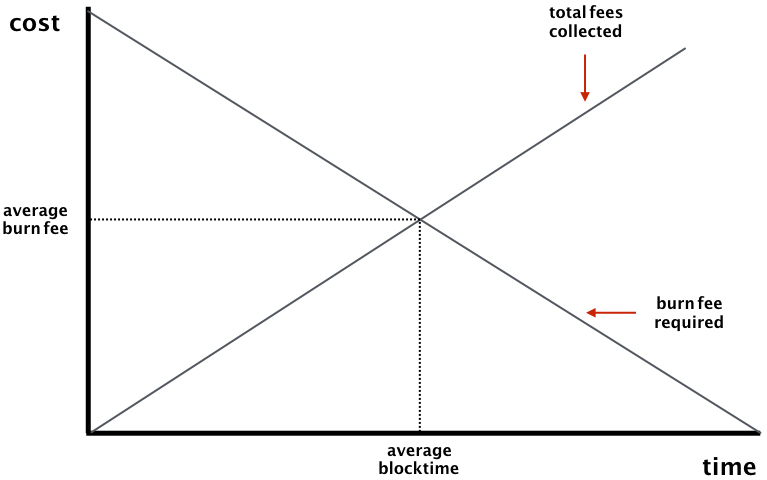
\includegraphics[width=.45\textwidth]{saito2.jpeg}

The burn fee makes attacking the network expensive, since any increase in the pace of block production requires attackers to have more transaction fees than the network is actually collecting. Honest nodes thus route transactions and produce blocks for free, while dishonest attackers can only launch temporary attacks on the network if they are willing to burn their own money to create fake transactions that include real fees. 

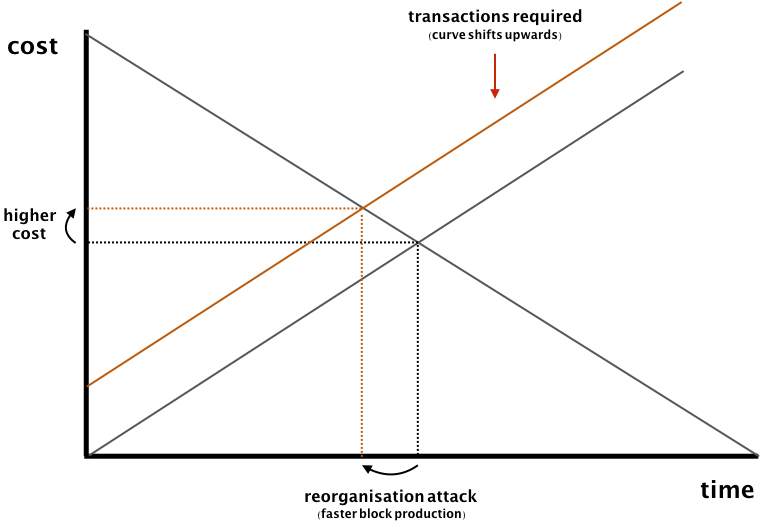
\includegraphics[width=.45\textwidth]{saito3.jpeg}

To further increase security, the Saito network has nodes sign transactions as they propagate them across the network, affixing to each an unforgeable history of its path from point of origin to point of confirmation. We require nodes to burn all fees from transactions that are not sent to them, and halve the percent of each fee that they can use to pay the burn fee with each hop a transaction has taken to reach them. along the network.

This allows the network to offer comparable security to Bitcoin in the sense that the cost of a chain-reorganization attack can always be quantified, and users that require significant guarantees that of non-reversibility can calculate the cost of a reorganization attack and wait for the appropriate number of confirmations.

There is one small problem with this approach:

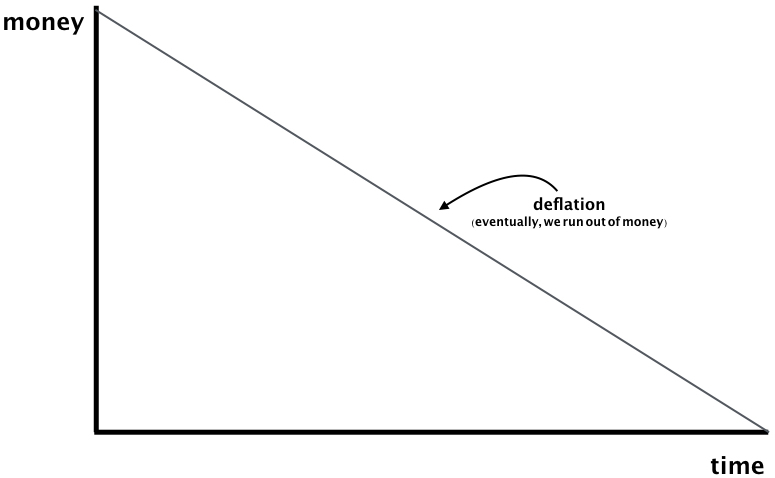
\includegraphics[width=.45\textwidth]{saito4.jpeg}

Constantly burning tokens will eventually cause a deflationary crash. To avoid this we must find a way to re-inject the lost tokens back into the network. Giving these tokens to productive nodes in the peer-to-peer network would be the ideal way to pay for bandwidth, but as long as the block-producing nodes have any influence over how funds are distributed a savvy attacker can game the system.

4. PAYING FOR BANDWIDTH

The solution is to introduce a second layer that randomizes payments while increasing network security. We achieve this by introducing a zero-sum competition between bandwidth-expending nodes and CPU-expending miners in the network. We call this battle for the "paysplit" of the network. It plays out as follows:

Whenever a node produces a block, it collects what profit it can and bundles its burned fees into a "golden ticket" that contains (1) a computational puzzle for miners to solve, and (2) a vote to increase, decrease, or hold constant the "paysplit" of the network (the percentage of all golden tickets that are paid out to miners). These tickets are included (by default) in all blocks produced. Miners listening on the network choose which blocks to solve and propagate solutions back into the network as regular fee-paying transactions. In addition to a proof-of-solution, these miner transactions also include a separate vote on whether to increase, decrease, or hold constant the difficulty of the computational puzzle.

The golden ticket system can be visualized as follows:

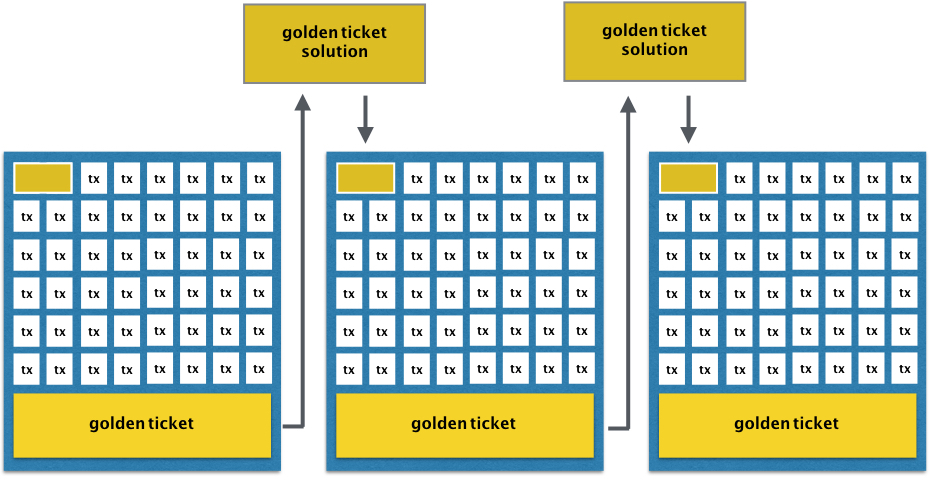
\includegraphics[width=.45\textwidth]{saito7.jpeg}

In order to increase the security of this method, we specify that only one solution may be provided for any golden ticket, and that solution must be included in the very next block. If these conditions are met, our two votes take effect, and the funds locked into the golden ticket are released to the network, split between the miner that found the solution and a random node in the peer-to-peer network. In the event a "golden ticket" is not solved it is not a problem either. The funds locked away will eventually fall off our transient blockchain, at which point they can be recycled back into our economy in another golden ticket.

This game is counterintuitive to most bitcoiners because it separates the act of "producing blocks" from the act of "getting paid". Also because all actors are trapped in a delicate dance requiring collusion and cooperation alike. For while both nodes and miners want at least one solution per golden ticket (because otherwise no-one gets paid), their interests otherwise diverge: miners prefer a high paysplit and high difficulty level, while nodes prefer a low paysplit and low difficulty level. Given that votes must pass between both players to change consensus settings, we end up with a competitive dynamic where agents in both groups are constantly trading-off their individual short-term against their collective long-term interests.

There are many obvious variants, such as the replacement of a mining puzzle with a proof-of-stake variant. The key observation is that full-nodes that have miner support will produce blocks at a faster rate and be more profitable than those who do not. And miners who have the support of full-nodes will also be more profitable. This creates a dynamic where excessive profits in any sector of the network (i.e. bandwidth provision) will attract competition that will support out-group actors in order to earn immediate supra-market profits. It is impossible without locking down the open access of the network, which is possible in other blockchains and guaranteed here by the fact that routing is incentivized.

This economic design makes the Saito Network robust and pushes us towards an equilibrium point at which the security provided is optimal for both nodes and miners given their relative ease of collusion and defection, something that is itself determined by the market structure surrounding the economics of bandwidth and security provision. A useful thought experiment is exploring how the security of this two-player system degrades to offer only bitcoin-level security as the paysplit approaches extreme values.

Since we acknowledge that this level is arbitrary and may not reflect the needs of the applications on the network, we allow users on the network to tag their transactions with an optimal paysplit vote. Should a user-originated transaction contain such a vote, our system insists that it can only be included in a block which votes in the same direction. Users who choose to take sides in the ongoing struggle between nodes and miners thus sacrifice the reliability and speed of transaction confirmation, but gain marginal influence over how the network allocates fees.

These simple rules combine to secure the Saito network against anti-social behaviors that are often not recognized as such in other blockchains. In Saito, for instance, transactions are naturally valuable to nodes which participate in the P2P network and useless to attackers who lurk on the edges. Fee-sourcing attacks and transaction theft are also impossible: the fact that nodes must participate in the P2P network to harvest transactions defends us against subtle attacks like the bitcoin FIBRE network, a closed-access network which benefits its participants by undermining the profitability of nodes which support the peer-to-peer network. And sibylling becomes an unprofitable strategy because it necessarily adds hops in transaction routes, making sibyls visible to other nodes and providing an evolutionary mechanism whereby weaker nodes which permit themselves to be sibylled necessarily lose revenue over time. 

Security is also reinforced by the competitive economic structure of our game in fascinating ways. Note that if network security falls too low, the network is incentivized to increase it by voting to pay miners more. How this secures the network is not obvious, but it does: greater pay for miners increases the amount needed to attack the network. A higher paysplit also supports the threatened chain in the long-run, and speeds up block-issurance through the higher fees miners pay for to have their solutions included over those of their peers. Even in situations where the network is not under active attack, the miner/node battle over the paysplit vote also serves a defensive "canary in the coalmine" function, encouraging miners to issue their own pro-miner blocks if they control enough hashpower to support the block.

5. SUMMARY

Saito is a solution for building a massively-scalable blockchain. We achieve this scalability not through algorithmic tweaks to existing technologies, but rather by solving the fundamental economic problems that characterize all existing consensus mechanisms.

Those who pour over the technical details of our consensus mechanism will find embedded in it at least six major innovations in blockchain technology: the transient blockchain, the burn fee, the usable transaction fee, the golden ticket system, the secure multi-party voting mechanism enforced by economic competition, and the chain of cryptographic signatures we embed in transactions that permits our network to identify and reward productive nodes in the network.  

We are keen for people to start building on Saito and welcome contact from other blockchain projects looking to incorporate one or several of these methods in their own networks. We have secured provisional patent protection and welcome the creation of a defensive alliance that allows us to share our own knowledge while ensuring that the technologies developed to build big-data applications cannot be perverted to undermine the free-speech values of the blockchain community.

We also encourage everyone to visit our website (http://saito.tech), where we maintain a working demo of the network, a roadmap outlining our development plans, links to downloadable software, and tutorials that can help anyone get started building Saito applications *today*. 

\end{multicols} 
\end{document}
